\documentclass[24pt, a2papper, portrait]{tikzposter}
\usepackage[utf8]{inputenc}

\title{Molecular computing}
\author{Alexander Aksentyev}
\date{\today}
\institute{National Research Nuclear University ``MEPhI''}

\usepackage{blindtext}
\usepackage{comment}
\usepackage{url}

\usetheme{Simple}

\begin{document}
	\maketitle
	
	\block{~}
	{
		Ever since the advent of the integrated circuit in the 1960s, computing has been synonymous with chips of solid silicon. But some researchers have been taking an alternative approach: building liquid computers using DNA and its cousin RNA, the naturally occurring nucleic-acid molecules that encode genetic information inside cells. Rather than encoding ones and zeroes into high and low voltages that switch transistors on and off, the idea is to use high and low concentrations of these molecules to propagate signals through a kind of computational soup.
	}
	
	\begin{columns}
		\column{0.5}
		\block{Silicon-based computers ...}{
			... use the semiconductor property of Silicon to encode information in \textbf{binary} (0,1) code.
			\begin{tikzfigure}
				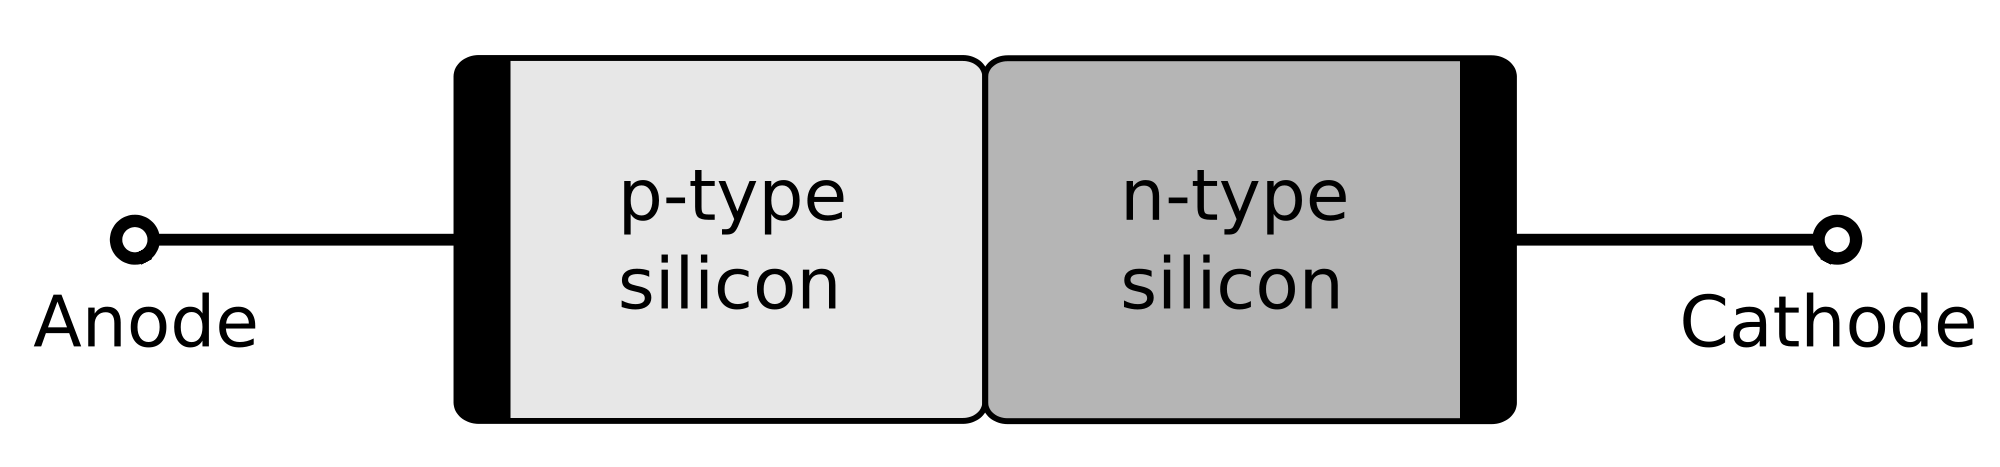
\includegraphics[width=.4\textwidth]{Diode}
			\end{tikzfigure}
		}	
		\block{A silicon computer chip ...}{
			... is made from a silicon crystal by introducing impurities (\emph{doping}).
			\begin{itemize}
				\item \textbf{N-type doping}: the silicon crystal is imbued with Phosphorous or Arsenic to add extra electrons.
				\item \textbf{P-type doping}: Boron or Gallium is the dopant. Each have only three electrons, hence when mixed into the silicon lattice they produce holes.
			\end{itemize}
			\begin{tikzfigure}
				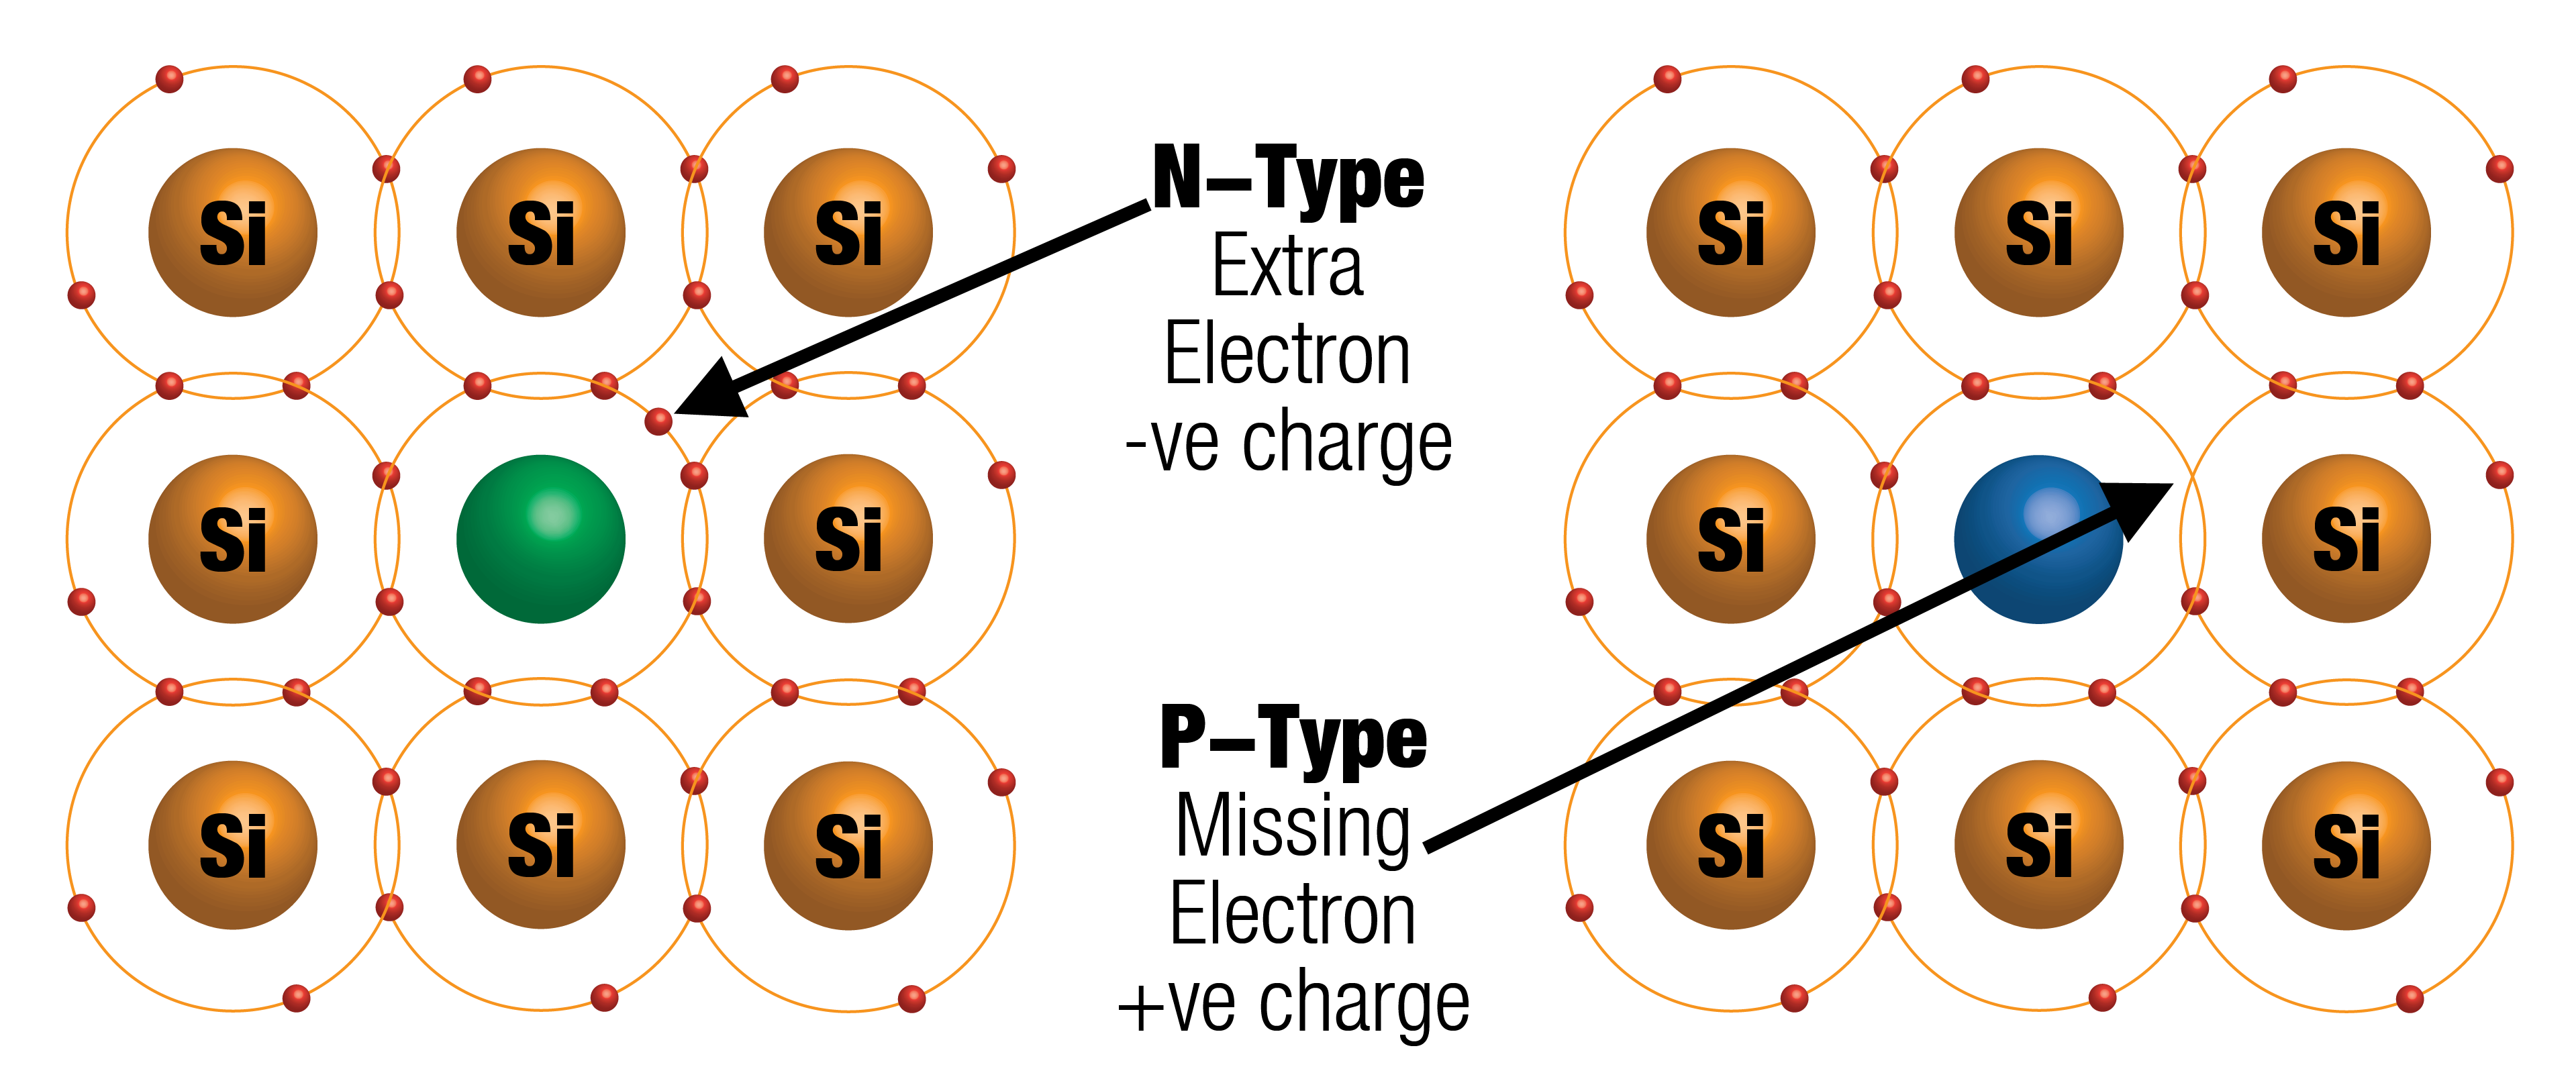
\includegraphics[width=.4\textwidth]{Si_chip_doped}
			\end{tikzfigure}
		}	
		\block{Moore's Law ...}{ 
			... predicts the number of transistors fitting on a computer chip.
			\begin{tikzfigure}
				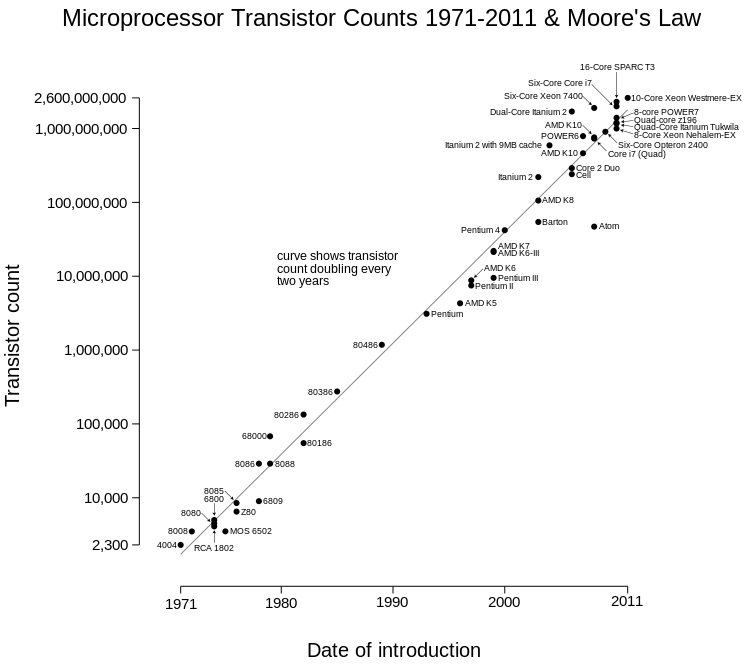
\includegraphics[width=.4\textwidth]{Moores_Law}
			\end{tikzfigure}
			Eventually, silicon-based microprocessors are bound to reach the limits of speed and miniaturization.
		}
		\column{0.5}
		\block{DNA-based computers ...}{
			... encode information in \textbf{quaternary} (A,T,C,G) code. Use biochemical reactions for computation.  
			\begin{tikzfigure}
				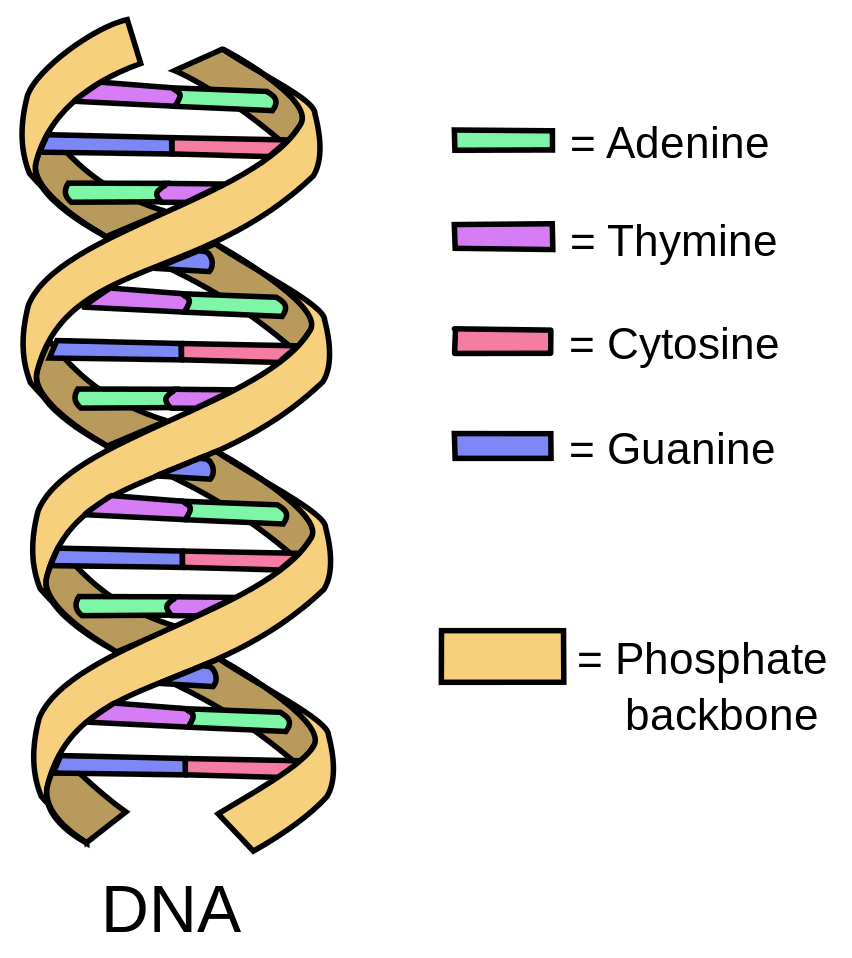
\includegraphics[width=.25\textwidth]{DNA_ATCG}
			\end{tikzfigure}
			\begin{itemize}
				\item \textbf{1 billion} times \emph{more} operations per Joule power than a silicon-based computer.
				\item \textbf{5 grams} of DNA can fit the \emph{Internet} \textbf{1000} times over.
				\item Each DNA strand is a microprocessor.
				\item AND, OR, NOT operations are performed by \emph{cutting}, \emph{linking}, \emph{pasting}, \emph{amplifying}, or \emph{repairing} DNA.
			\end{itemize}
		}
		\block{A biochip ...}{
			... is a miniaturized laboratory that can perform \textbf{100,000} simultaneous biochemical reactions. Biochips are fabricates in \textbf{two} ways:
			\begin{itemize}
				\item In \textbf{Microarrays}, a 2D array of \textbf{DNA} or \textbf{proteins} is arranged on a solid substrate.
				\item In \textbf{Microfluidics}, the behavior of biological fluids is precisely controlled by micro pumps and micro valves. 
			\end{itemize}
			\begin{tikzfigure}
				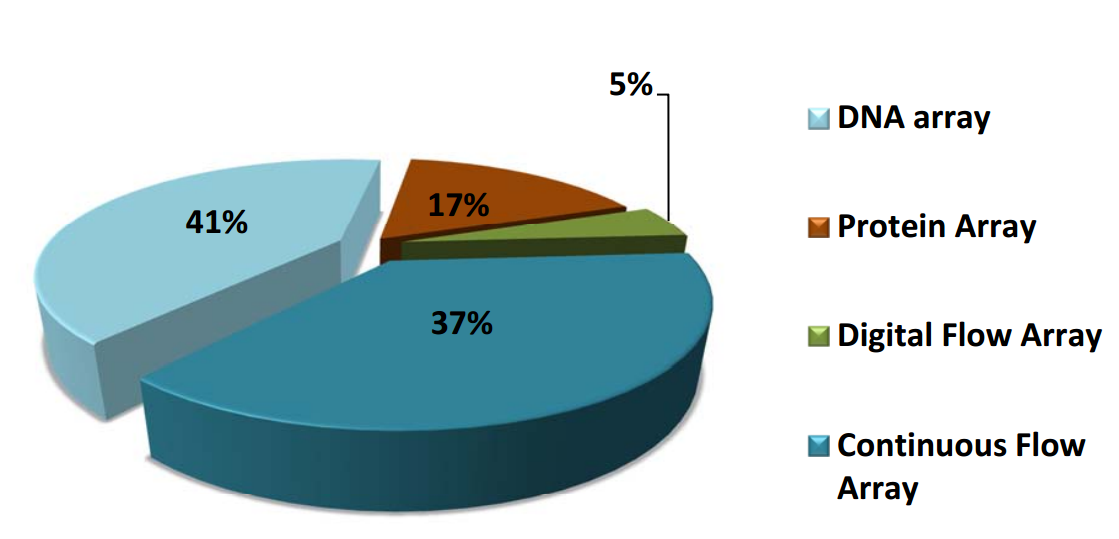
\includegraphics[width=.4\textwidth]{Biochip_Fabrication_Types}
			\end{tikzfigure}
		\begin{itemize}
			\item \textbf{Continuous Flow} arrays manipulate continuous liquid in micro fabricated channels.
			\item In \textbf{Digital Flow} arrays, discrete and independently controlled droplets are manipulated on a substrate using electro wetting.
		\end{itemize}
		}
		\block{Pros and Cons}{
			\begin{minipage}[t]{.22\textwidth}
				\begin{itemize}
					\item \textbf{Millions} of operations simultaneously
					\item Generate a complete set of potential solutions
					\item Could be made small enough to operate inside cells and control their activity
					\item Efficiently handle massive amounts of working memory
				\end{itemize}
			\end{minipage}~
			\begin{minipage}[t]{.22\textwidth}
				\begin{itemize}
					\item Biochemical reactions take anywhere from minutes to days to complete
					\item Generation of solution sets may require impractical amounts of memory
				\end{itemize}
			\end{minipage}
		}
	\end{columns}

	
\end{document}